% !TeX program = xelatex
% !TeX encoding = UTF-8
\documentclass[UTF8]{standalone}
\usepackage{amsmath,fourier,ctex,tikz,upgreek}
\begin{document}
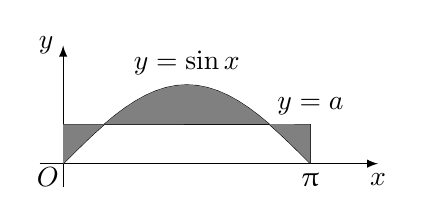
\begin{tikzpicture}[domain=-0.3:3]
	\draw[-latex] (-0.3,0) node[left=-3pt,below=-2pt] {$O$} -- (4,0) node[below] {$x$};
	\draw[-latex] (0,-0.3) -- (0,1.5) node[left] {$y$};
	\draw[domain=0:3.14] plot (\x,{sin(\x r)}) node[below] {$\uppi$};
	\node[above] at (1.57,1) {$y = \sin x$};
	\draw (0,0.5) -- (3.14,0.5) node[above] {$y = a$} -- (3.14,0);
	\fill [fill = gray] [domain = 0:0.52333,smooth] plot (\x, {sin(\x r)}) -- (0,0.5) -- cycle;
	\fill [fill = gray] [domain = 0.52333:2.61666,smooth] plot (\x, {sin(\x r)})  -- cycle;
	\fill [fill = gray] [domain = 2.61666:3.14,smooth] plot (\x, {sin(\x r)}) -- (3.14,0.5) -- cycle;
\end{tikzpicture}
\end{document}